%%%%%%%%%%%%%%%%%%%%%%%%%%%%%%%%%%%%%%%%%%%%%%%%%%%%%%%%%%%%%%%%%%%%%%%%%%%%%%%%%
% Introducción
%%%%%%%%%%%%%%%%%%%%%%%%%%%%%%%%%%%%%%%%%%%%%%%%%%%%%%%%%%%%%%%%%%%%%%%%%%%%%%%%%

\chapter{Introducción} % (fold)
\label{cha:Introduccion}

    \section{Historia de los instrumentos digitales} % (fold)
    \label{sec:HistoriaDeLosInstrumentosDigitales}

        Los primeros intentos de guardar y reproducir el sonido fueron analógicos. Estos métodos captan las ondas y las
        almacenan en diferentes medios para su posterior reproducción, como en un disco de vinilo o un casete.

        Con la aparición de la informática y los ordenadores se empiezan a almacenar estos sonidos en un formato
        digital, capaz de ser interpretado por ordenadores. En este caso, los sonidos se guardan en forma de bytes en
        diferentes formatos de archivo, como MP3, AAC, OGG...

        Los primeros intentos de instrumento musical no analógico se pueden encontrar en los sintetizadores. Estos
        intrumentos utilizan la electricidad para producir las ondas del sonidos pasándola por una serie de módulos.
        Hasta la década de 1980, cada fabricante utilizaba su propio estándar para la sincronización de los sonidos de
        los sintetizadores. En 1981, la empresa Oberheim Electronics comenzó a contactar con otros fabricantes para
        desarrollar un estándar, de ese modo apareció MIDI. Este estándar describe el protocolo de comunicación, la
        interfaz digital y las conexiones electrónicas que deben llevar los diferentes tipos de dispositivos
        electrónicos para reproducir, editar y grabar música \cite{midi_wikipedia}.

        En cuanto a instrumentos musicales electrónicos podemos encontrar desde un teclado o una guitarra a una batería.

        En el área de instrumentos digitales nos encontramos con los instrumentos VST (Virtual Studio Technology). Estos
        instrumentos toman muestras de sonidos de diferentes instrumentos y, mediante un teclado y un ordenador,
        programar estos sonidos y componer y grabar cualquier tipo de canción \cite{historia_instrumentos_digitales}.
        
        \newpage

        \begin{figure}[ht]
            \centering
            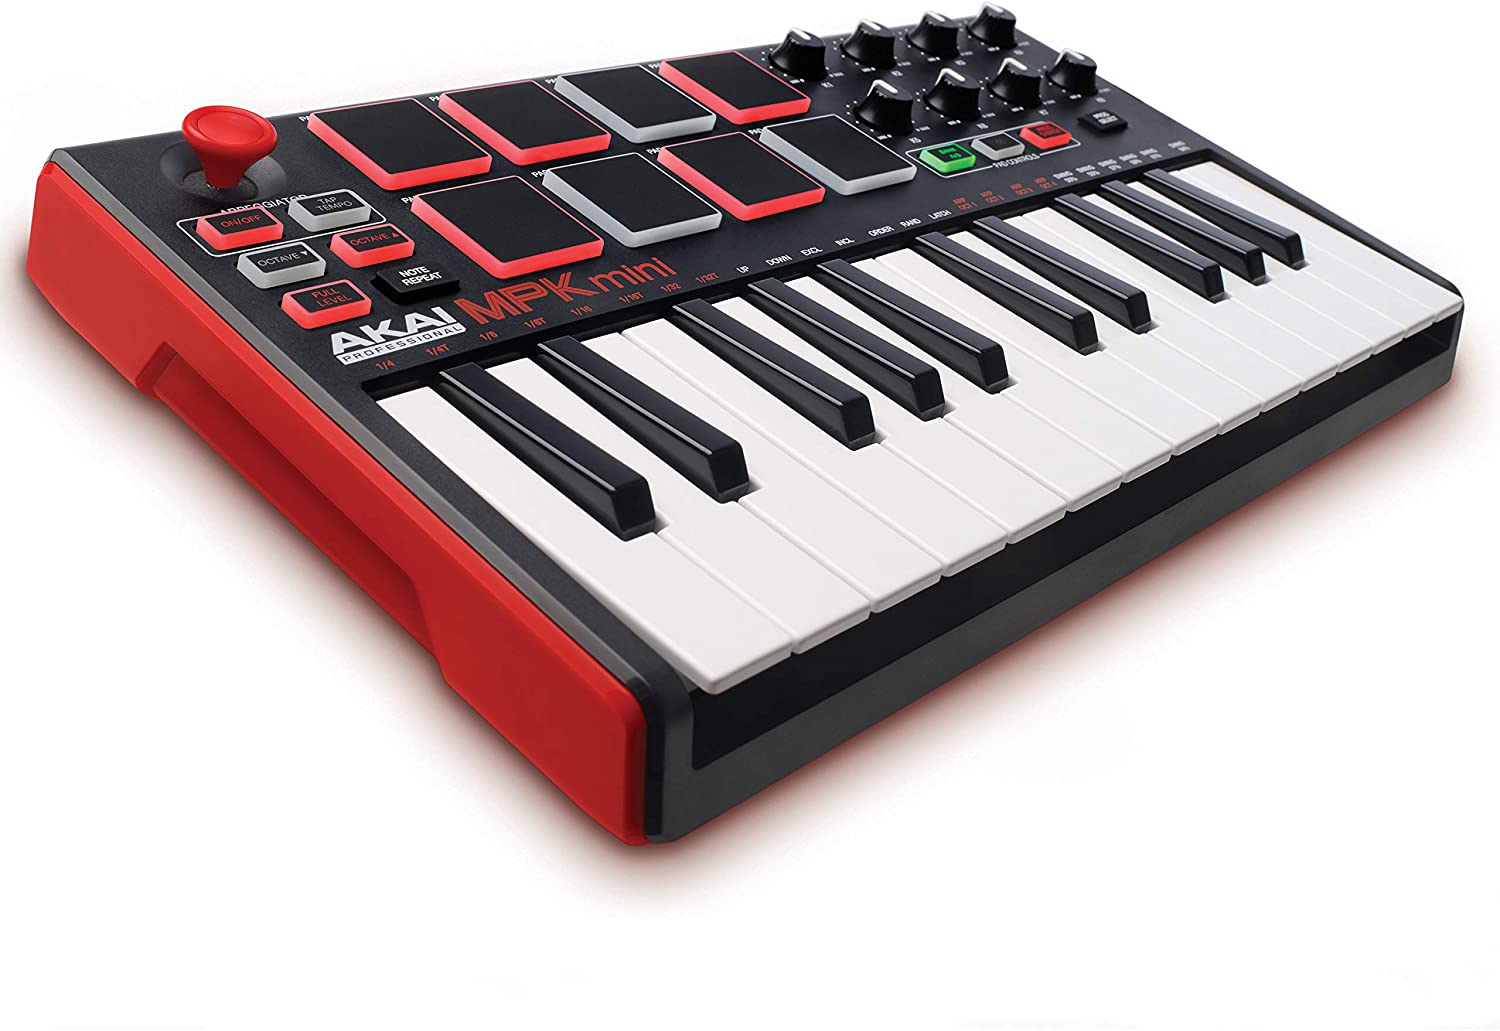
\includegraphics[width=\textwidth/2]{ejemplo_sampler}
            \caption{Ejemplo de sampler digital de la marca AKAI Pro \cite{akai_pro_imagen}\label{fig:EjemploSampler}}
        \end{figure}

    % section Historia de los instrumentos digitales (end)

    \section{Partes de una batería} % (fold)
    \label{sec:PartesDeUnaBateria}

        Las partes de una batería son las siguientes:

        \begin{itemize}
            \item \textbf{Caja}: Su función principal suele ser la de marcar los compases.
            \item \textbf{Toms}: Son los tambores más numerosos en una batería.
            \item \textbf{Bombo}: Se toca con un pedal y produce el sonido más grave de la batería. Se utiliza para
            llevar la base del ritmo.
            \item \textbf{Platillo crash}: Se utiliza para dar énfasis y suele ir acompañado del bombo.
            \item \textbf{Platillo hi-hat}: Consta de dos platillos que se pueden abrir o cerrar con un pedal y se
            utiliza para llevar el ritmo de la canción.
            \item \textbf{Platillo ride}: Puede usarse para llevar el ritmo en lugar de con el hi-hat.
        \end{itemize}
        
        \newpage

        \begin{figure}[ht]
            \centering
            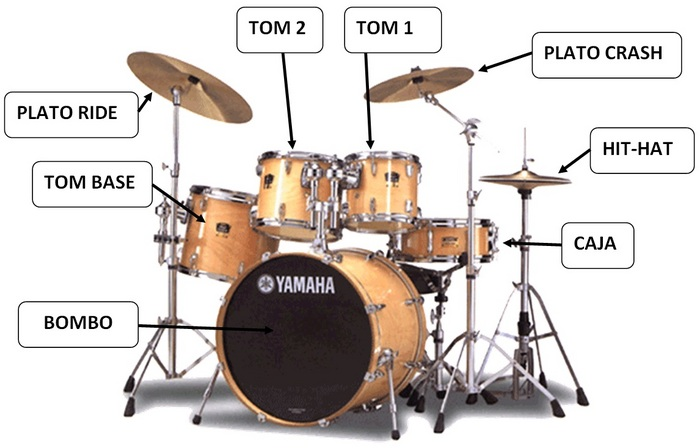
\includegraphics[width=10cm]{partes_bateria}
            \caption{Partes de una batería \cite{partes_bateria_fuente}\label{fig:PartesBateria}}
        \end{figure}

    % section Partes de una batería (end)
    
    \section{Etapas} % (fold)
    \label{sec:Etapas}

        \begin{itemize}
            \item \textbf{1ª etapa:} Estudio del problema.

            \item \textbf{2ª etapa:} Búsqueda de bibliotecas de reproducción de sonido.

            \item \textbf{3ª etapa:} Implementación del software.

            \item \textbf{4 a etapa:} Construcción de la batería.

            \item \textbf{5ª etapa:} Documentación.
        \end{itemize}

    % section Etapas (end)

    \section{Planificación} % (fold)
    \label{sec:Planificacion}

        \subsection{A priori optimista} % (fold)
        \label{sub:APrioriOptimista}

            \begin{figure}[ht]
                \centering
                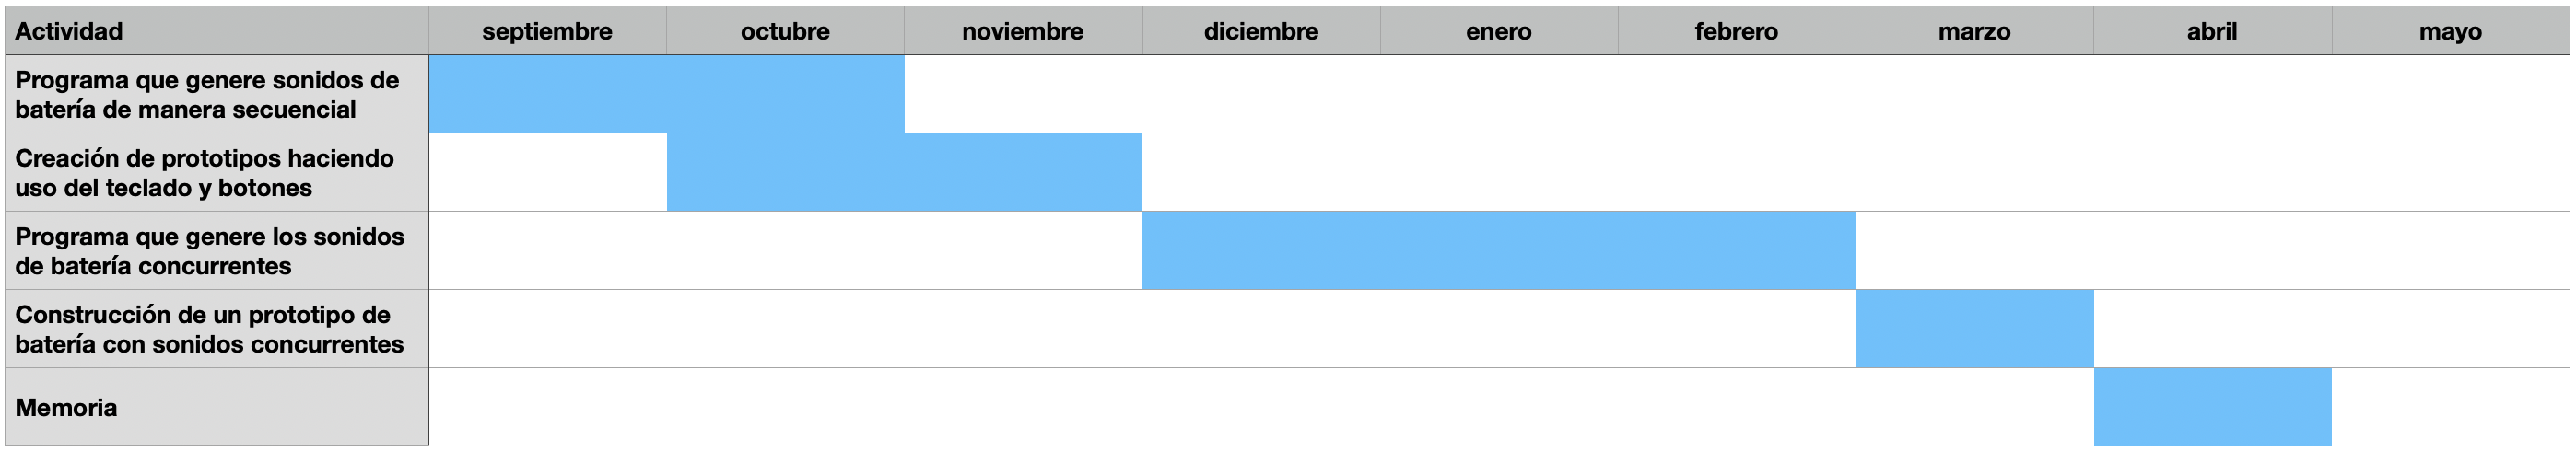
\includegraphics[width=\textwidth]{planificacion_gantt}
                \caption{Diagrama de Gantt de la planificación por etapas\label{fig:PlanificacionGantt}}
            \end{figure}

        % subsection A priori optimista (end)

        % \subsection{A posteriori (en caso de haber diferencias)} % (fold)
        % \label{sub:APosterioriEnCasoDeHaberDiferencias)}

        % subsection A posteriori (en caso de haber diferencias) (end)

    % section Planificación (end)

% chapter Introducción (end)

\newpage